%In dit hoofdstuk moet het volgende besproken worden:
%-Uitleggen van het probleem
%-Hoe ik tewerk ga gaan
%-Gaan we concluderen met de onderzoeksvraag
\chapter{Inleiding}\label{hfdst:situering}
\section{Situering}
%%% TODO meer schrijven over wat televic rail doet en wat zij maken -> uitleggen dat framework daarbij te pas komt
%http://www.railway-technology.com/contractors/operation/televic-rail/
Met meer dan 30 jaar ervaring in het ontwerpen en onderhouden van on-board communicatiesystemen is Televic Rail een toonaangevende producent van Passenger Information Systems, Entertainment Systems and Infotainment Systems.
LiveCom is Televic Rail nieuwste generatie van informatiemanagement systemen.
Het integreert alle aspecten van de on- en off-board reizigersinformatie, de infotainment en de entertainment. 
Het stelt operatoren in staan om hun volledige verkeersschema's, de dienstregelingen, de routes, de stations en alles met betrekking tot informatie en infotainment omtrent passagiers te beheren, met behulp van off-board software tools.

iCoM, de geïntegreerde oplossing van Televic Rail voor passagiersgegevens en communicatiemanagement, biedt het openbaar vervoer en spoorwegondernemingen een centraal systeem voor het creëren, het beheren, het distribueren en het uitvoeren van real-time on en off-board generieke en commerciële passagiersinformatie op de vloot, in stations en bij haltes.

Naast deze systemen heeft Televic verschillende mechatronica-sensoren en veiligheid controlesystemen ontworpen.
Alle systemen en apparaten zijn ontworpen in overeenstemming met de betreffende spoorwegsectornormen en voldoen aan de eisen voor passagiersruimte, draaistel en asmontage. 
On-board controllers verwerken sensordata-informatie en sturen deze naar de betreffende actuators en treinbeheersingssystemen.
Fysische parameters die momenteel worden ondersteund zijn onder andere de versnelling, de druk, de rotatie, de temperatuur, het geluid en de verplaatsing.

Om te voldoen aan de strenge veiligheidsnormen heeft Televic Rail een Python test framework ontworpen waarmee Televic in staat is om verschillende producten te onderwerpen aan verschillende testscenario's.
Het framework werd ontworpen om gebruikt te worden op specifieke testtorens en werd later aangepast om bruikbaar te zijn op gewone computers.
Dit framework wordt intensief gebruikt tijdens het productieproces en is cruciaal voor het afleveren van producten die voldoen aan de strenge veiligheidsnormen.

\section{Probleemstelling}\label{sec:probleem}
Het Python testraamwerk moet correct functioneren met een grote hoeveelheid producten van Televic.
Hierdoor gebruikt het Python testraamwerk verschillende drivers en bibliotheken.
Een direct gevolg hiervan is dat het installatieproces tijdrovend en foutgevoelig is.
Verder dient elk nieuw toestel op het raamwerk ondersteunt te worden waardoor er jaarlijks vele releases van het raamwerk verspreid worden.
Het installatieproces en het updateproces vragen om een vereenvoudiging zodat het testraamwerk gebruiksvriendelijker wordt.

Doordat het installatieproces en het updateproces foutgevoelig zijn, moet een ``rampenplan'' voorzien worden.
Door de aanwezigheid van een ``rampenplan'', worden mogelijke fouten vermeden en indien nodig opgevangen en verholpen.
Zo wordt vermeden dat de productielijn moet worden stilgelegd door bijvoorbeeld een fout tijdens het updaten van een applicatie.
Het is dus belangrijk dat applicaties op een eenvoudige manier geïnstalleerd en geüpdatet kunnen worden op verschillende hardware.
Om dit te laten slagen moet het testraamwerk eerst bij de verschillende doelsystemen geraken.
Er zullen dus producenten van software zijn die de verschillende testraamwerken produceren en willen verspreiden maar ook gebruikers die deze willen ontvangen.
Het proces waarbij software van een producent naar alle toepasbare gebruikers verspreid wordt en vervolgens geïnstalleerd wordt, wordt ook wel het deployment proces genoemd.
Een schets is zichtbaar in Figuur~\vref{fig:simpleServerClient}.

\begin{figure}[!ht]
\centering
\makebox[0pt]{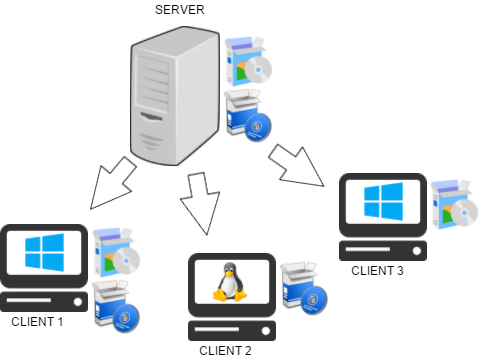
\includegraphics[scale=0.7]{afbeelding/simpelServerClient.png}}
\caption{Voorstelling van software verspreiding}
\label{fig:simpleServerClient}
\end{figure}

Tijdens het zoeken naar een oplossing voor het installatieproces en updateproces van het Python testraamwerk, moet gezocht worden naar een oplossing die ook antwoorden biedt op toekomstige problemen.
Tot op heden werd ervan uitgegaan dat de enige applicatie die moet verspreid, geïnstalleerd en geüpdatet worden het Python testraamwerk is.
In de toekomst moet het echter mogelijk zijn om verschillende applicaties te ondersteunen.
Het is dan ook belangrijk dat een oplossing gevonden wordt die een groeiend aantal gebruikers ondersteund.
Naargelang het aantal applicaties die ondersteund worden stijgt, zullen meer systemen gebruik maken van de applicatie.
Naarmate het aantal gebruikers stijgt, stijgt ook de vraag naar een algemene administratieve interface. 
Met een administratie interface wordt het mogelijk om bij te houden hoe het uitrollen van een nieuwe versie van een applicatie verloopt.
Deze informatie kan gebruikt worden om het verspreidingsproces bij te sturen zodat een volgende keer het proces vlotter verloopt.
Naast het ondersteunen van verschillende applicatie moet tijdens het ontwerpen rekening gehouden worden met verscheidene besturingssystemen.
De huidige programma's draaien op Windows maar het gebruik van Linux of andere systemen is in de toekomst niet uit te sluiten.

Het doel van deze thesis is dan ook een oplossing te vinden voor het complexe installatieproces en updateproces.
Daarbij moet de software eerst van de producent bij de gebruikers geraken en moeten deze processen rekening houden met een ``rampenplan'' om fouten tijdens een installatie of update op te vangen.
Verder wordt tijdens de ontwerpfase van de applicatie rekening gehouden met een groeiend aantal applicaties die verspreid en geïnstalleerd moeten worden, een groeiend aantal gebruikers die deze applicaties willen ontvangen en de diversiteit van besturingssystemen van deze gebruikers.

\section{Overzicht}
Het tweede hoofdstuk bevat een literatuurstudie over het deployment probleem.
Er wordt nagegaan welke architecturen en technologieën beschikbaar zijn om de verschillende deelproblemen op te lossen.

Vervolgens vindt in het derde hoofdstuk een bespreking plaats van de ontworpen architectuur.
In dit hoofdstuk wordt toegelicht waarom bepaalde architecturen en technologieën gekozen worden.
Vervolgens wordt besproken hoe de verschillende architecturen en technologieën gecombineerd worden tot één geheel die de basis vormt voor de implementatie.

In het vierde hoofdstuk worden implementatiekeuzes toegelicht en soms uitgediept.

In hoofdstuk vijf wordt de ontworpen applicatie onderworpen aan verscheidene scenario's om te achterhalen of de applicatie voldoet aan de verwachtingen.
Hierna volgt een SWOT analyse om na te gaan wat de sterktes en zwaktes zijn van de applicatie.

